\subsection{Perch Detection Software Design}

The image processing software used to validate the perch detection concept was implemented in C++ and executed on a Raspberry Pi Compute Module 4. The graph in figure 
\ref{fig:sw-flow} provides a high-level illustration of the steps in the image processing pipeline and how data flows between them.

\begin{figure}[H]
    \centering
    \digraph[width=\textwidth]{swflow}{
        rankdir=TB;
        lc [label="Left Camera Frame Acqusision" shape=box];
        rc [label="Right Camera Frame Acqusision" shape=box];
        ls [label="Left Stereo Block Matching" shape=box];
        rs [label="Right Stereo Block Matching" shape=box];
        f [label="Weighted Least Squares Filtering" shape=box];
        pc [label="Point Cloud Projection and Downsampling" shape=box];
        ht [label="3D Hough Transform" shape=box];
        s [label="Best Candidate Selection" shape=box];

        lc -> ls [label="Left Side Image"];
        lc -> rs [label="Left Side Image"];
        lc -> f [label="Guide For Inpainting"];
        rc -> ls [label="Right Side Image"];
        rc -> rs [label="Right Side Image"];
        ls -> f [label="Left-To-Right Disparity"];
        rs -> f [label="Right-To-Left Disparity"];
        f -> pc [label="Filtered Disparity and Confidence Map"];
        pc -> ht [label="Down-Sampled Point Cloud"];
        ht -> s [label="Position, Orientation, and Dimensions of Candidate Lines"];        
    }
    \caption{Diagram of the dataflow for the proposed image processing pipeline, starting from image aquisition on the top
        to generation of coordinates for the detected perch on the bottom.}
    \label{fig:sw-flow}
\end{figure}



\subsection{Stereo Camera Calibration}

A camera calibration script was creates using the functions available in OpenCV \cite{bradski_opencv_2000}. The script can be read in appendix \ref{app:cal-code}.
285 total calibration image pairs were captured. The calibration pattern used was an 8 marker by 11 marker ChArUco board with 20mm checkers and 15mm markers, and a 4x4 AruCo dictionary.

To perform individual camera intrinsic and distortion parameter calibrations, each image was loaded and the pattern corners were detected and mached to the expected board layout.
Any image in which fewer than 10 corner points were detected was discarded, as low point counts can result in bad calibration parameters. For accepted images, the identified calibration
pattern corner locations in the image coordinates are saved, as well as the estimated position and orientation of the calibration board. The accepted points were then used to calculate 
an initial estimate of the cameras intrinsic matrix and distotion coefficients. The calibration at this point is still low quality, so an iterative refinement is now applied. For each image
that was not rejected, the calibration pattern points are projected into image coordinates using the saved position and orientation estimates of the calibration board. Then the error between these 
projected points and the positions of the previously detected points in that image were calculated. Once these errors were calculated for all images, any point in an image that had a reprojection error 
greater than 3 standard deviations of the reprojection error for all points in all images was discarded, under the assumption that this high error was due to a bad detection of that corner. If any image 
contained less then 10 valid points after removing points with high error, the entire image was discarded. This process was repeated until either one of the following termination criteria was met:

\begin{itemize}
    \item The change in standard deviation of the reprojection errors for all points in all images was less than $1e-9$.
    \item The iteration limit of $5$ was reached.
\end{itemize}


The stereo translation and rotation parameter calibration process followed a similar design, however in the initial filtering and later iterative remove, only points 
that were valid in both images were retained (ChArUco patterns use QR-like codes that allow points to be identified uniquely across different images or in partial occlusions).
So if calibration point A was detected in the left image but not in the right image, or if it was detected in both but then was removed from the left point set due to too high 
reprojection error, then it was not used in either. Image pairs that had less than 10 valid points in either left or right image were rejected from both sets. 

After following this process for each individual camera, and then for the stereo combination, 26 images were retained as valid for the left camera, 17 for the right camera, and 
10 images retained for the stereo combination. A visual inspection of the reprojection errors and detected corner locations was performed to confirm that:

\begin{itemize}
    \item The errors were approximately zero-mean.
    \item The errors had approximately the same distribution in the x and y directions.
    \item The detected marker locations covered most of the camera frame, to avoid overfitting to non-symetrical lens defects on one portion of the image. 
\end{itemize}

Figures \ref{fig:cal-left}, \ref{fig:cal-right}, and \ref{fig:cal-stereo} show the visualizations used to perform this inspection of calibration results.

\begin{figure}[H]
    \centering
    \begin{subfigure}[b]{0.45\textwidth}
        \centering
        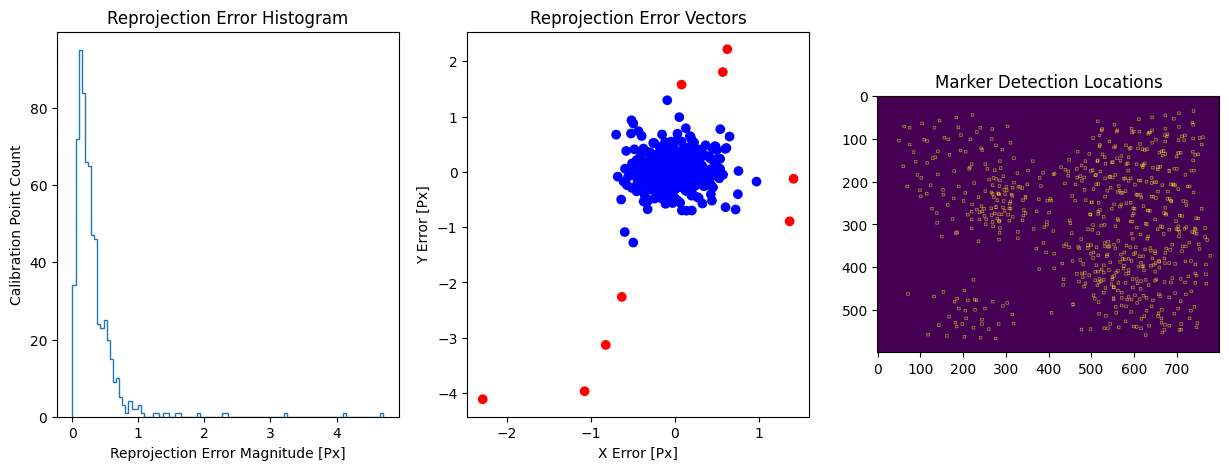
\includegraphics[width=\textwidth]{sections/methods/left-cal-pre.png}
        \caption{Before removing outliers.}
        \label{fig:cal-left-1}
    \end{subfigure}
    \vfill
    \begin{subfigure}[b]{0.45\textwidth}
        \centering
        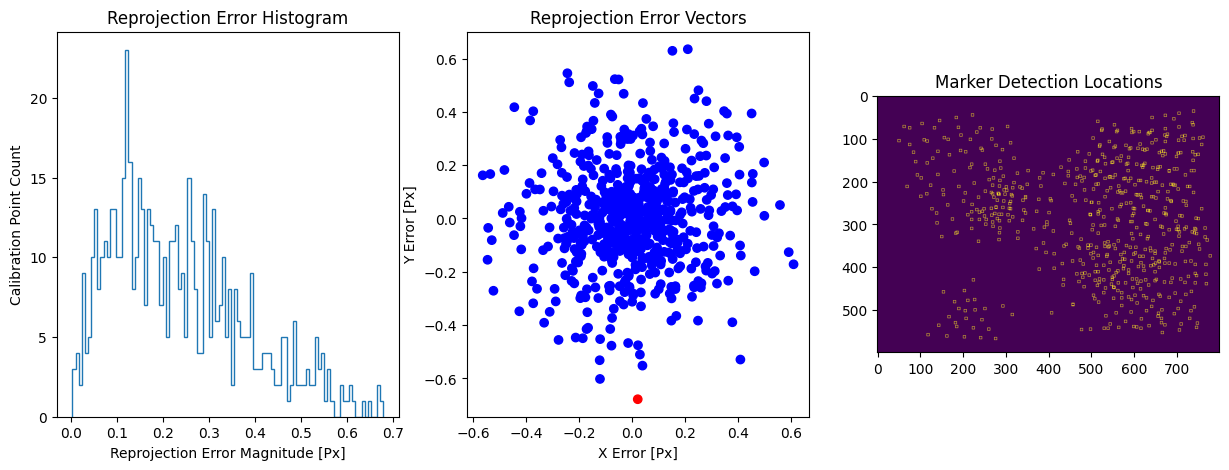
\includegraphics[width=\textwidth]{sections/methods/left-cal-post.png}
        \caption{After removing outliers.}
        \label{fig:cal-left-2}
    \end{subfigure}
    \caption{Calibration visualizations for the left camera, before (\ref{fig:cal-left-1}) and after (\ref{fig:cal-left-2}) iterative outlier removal.}
    \label{fig:cal-left}
\end{figure}

\begin{figure}[H]
    \centering
    \begin{subfigure}[b]{0.45\textwidth}
        \centering
        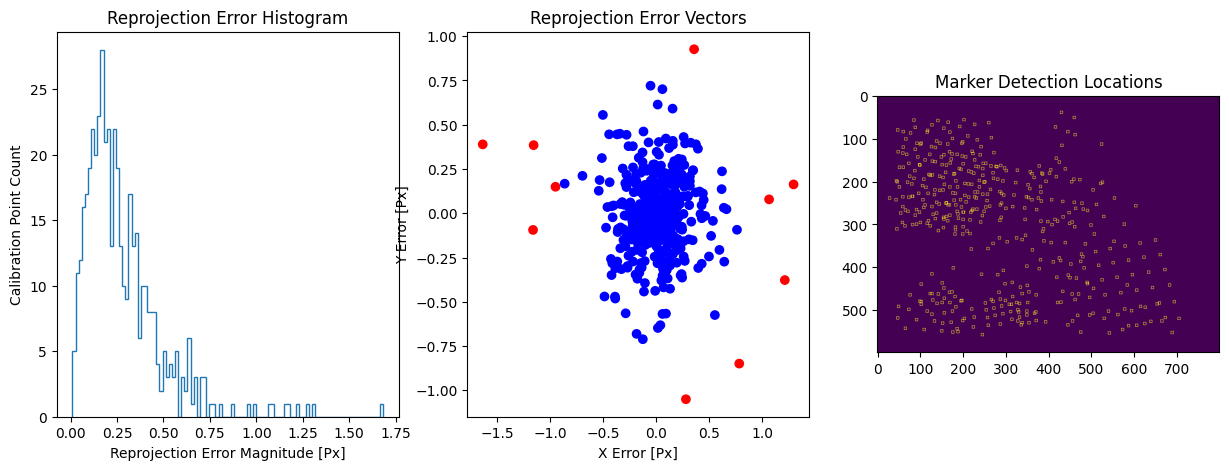
\includegraphics[width=\textwidth]{sections/methods/right-cal-pre.png}
        \caption{Before removing outliers.}
        \label{fig:cal-right-1}
    \end{subfigure}
    \vfill
    \begin{subfigure}[b]{0.45\textwidth}
        \centering
        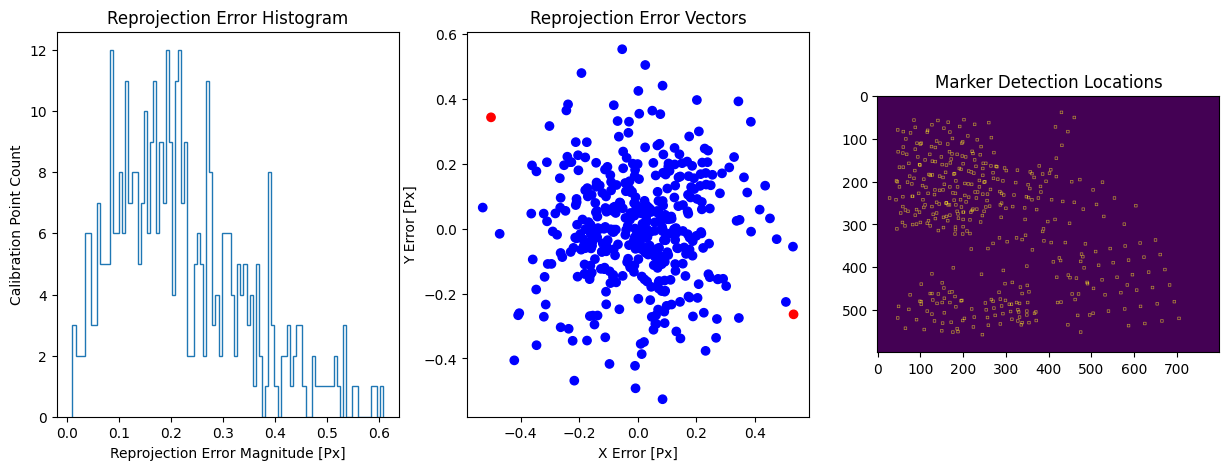
\includegraphics[width=\textwidth]{sections/methods/right-cal-post.png}
        \caption{After removing outliers.}
        \label{fig:cal-right-2}
    \end{subfigure}
    \caption{Calibration visualizations for the right camera, before (\ref{fig:cal-right-1}) and after (\ref{fig:cal-right-2}) iterative outlier removal.}
    \label{fig:cal-right}
\end{figure}

\begin{figure}[H]
    \centering
    \begin{subfigure}[b]{0.45\textwidth}
        \centering
        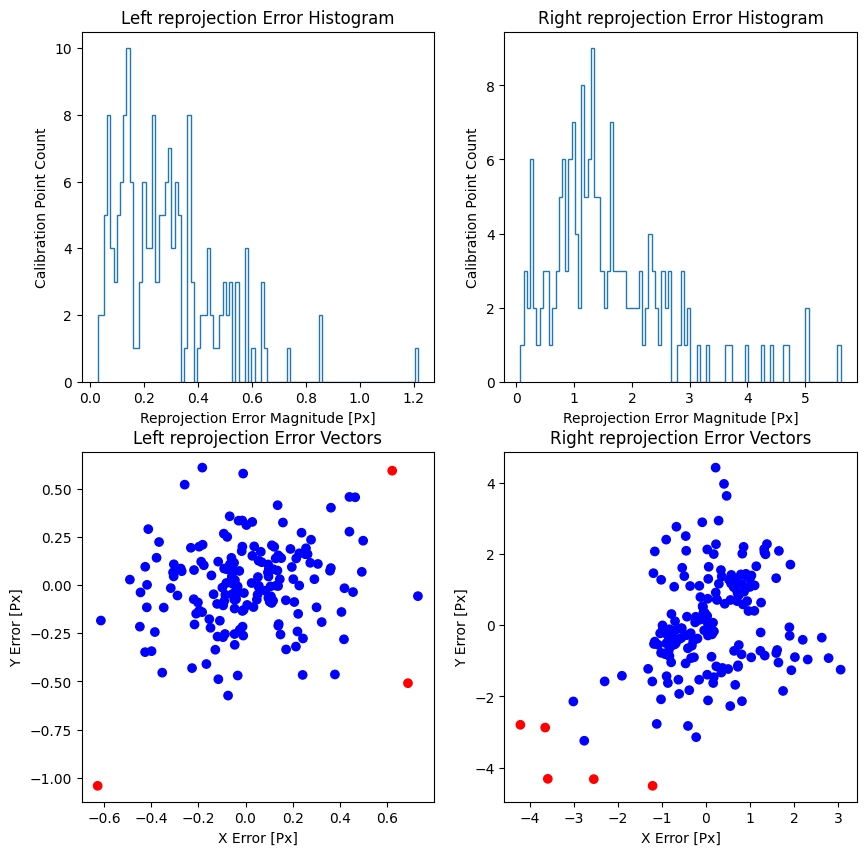
\includegraphics[width=\textwidth]{sections/methods/stereo-cal-pre.png}
        \caption{Before removing outliers.}
        \label{fig:cal-stereo-1}
    \end{subfigure}
    \vfill
    \begin{subfigure}[b]{0.45\textwidth}
        \centering
        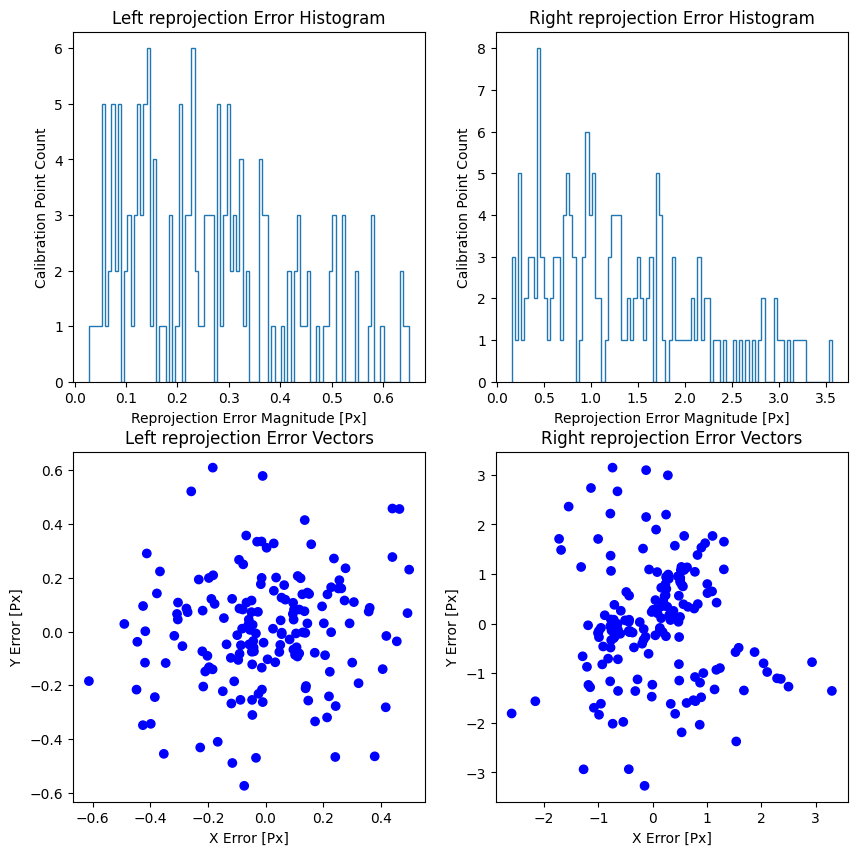
\includegraphics[width=\textwidth]{sections/methods/stereo-cal-post.png}
        \caption{After removing outliers.}
        \label{fig:cal-stereo-2}
    \end{subfigure}
    \caption{Calibration visualizations for the stereo pair, before (\ref{fig:cal-stereo-1}) and after (\ref{fig:cal-stereo-2}) iterative outlier removal.}
    \label{fig:cal-stereo}
\end{figure}

\subsection{Perch Detection Validation Data Collection}

To first test the detection methods performance under the most controlled conditions, the device was placed facing a flat white wall, indoors,
with only one object (a gray, 15mm diameter PVC pipe) in the frame. The object was placed at a distance $d = 1000mm$ from the camera, at an azimuth angle (angle between
object and cameras y axis) $\theta = 0^\circ$ and elevation angle (angle between the cameras x-y plane and the object) $\phi = 0^\circ$.

The image processing program was started by the script found in appendix \ref{app:data-coll-code}. Once the output of the program indicated that at least one
candidate line had been detected, the program was run for 2 minutes. The script monitored the detection results via serial terminal and saved the position, 
orientation, and dimensions of the detected object each time a new update was produced by the detection program. At each new update the script also triggered the
program to save a binary file containing both left and right images, the calculated disparity and confidence map, the filtered point cloud, and information about the 
identified line candidates with labels for all points in the point cloud that belong to a line canditate.

This test was performed for the following combinations of object poses. All angles were measured to be within $5^\circ$ of the target value using the "Clinometer" Android app,
and the distances measured within $5mm$ via tape measure.

\begin{itemize}
    \item $d = 5000mm$, $\theta = 0^\circ$, $\phi = 0^\circ$
    \item $d = 1000mm$, $\theta = 0^\circ$, $\phi = 0^\circ$
    \item $d = 2000mm$, $\theta = 0^\circ$, $\phi = 0^\circ$
\end{itemize}

These three trials were then repeated with the object in front of a zig-zag background pattern. The motivation for this test is to compare the success rate in best and worst case conditions; the 
flat white wall tends to be the most difficult case for the detection process due to the lack of features for stereo matching to use. The zig-zag background serves as a more optimistic performance test.

A review of initial results showed that the performance against the white wall background was poor. A possible method to improve this is to threshold the left image into light and dark regions, and
only include points whose color falls in the dark region in the point cloud. This assumes that the target object will always be darker than the background. For a perching device facing upward towards
open sky or tree canopies, this assumption may hold true. To implement this the "Weighted Least Squares Filtering" in figure \ref{fig:sw-flow} was modified to include the following algorithm:

\begin{enumerate}
    \item A Gaussian blur with a 5x5 kernel is applied to the left camera image.
    \item A threshold value is determined for the blurred image via Otsu's method.
    \item For each pixel with an intensity greater than the threshold value, the corresponding disparity value is set to -1. 
        Negative disparity values result in invalid points whcih get filtered out in the "Point Cloud Projection and Downsampling" step of figure \ref{fig:sw-flow}
\end{enumerate}

This was tested again with both white and zig-zag backgrounds. The tests with added threshold filtering were performed by processing saved data from the first test trials through the
image processing pipeline rather than collecting new data. The script in appendix \ref{app:retest-code} was used to process this new test data.

Table \ref{tab:vision-test-cases} shows all test cases that were perform.

\begin{table}[H]
    \centering
    \caption{List of test scenarios for which data was collected.}
    \label{tab:vision-test-cases}
    \begin{tabular}{c|cc}
        Case Number & Background Type & Threshold Based Filter \\
        \hline
        1 & White & Off  \\
        2 & Zig-Zag & Off \\
        3 & White & On \\
        4 & Zig-Zag & On
    \end{tabular}
\end{table}

\subsection{Perch Detection Validation Data Analysis}

The first analysis performed on the detection data was determining how often the device correctly detected the object. This 
was done using the binary files saved in the data collection process alongside the script in appendix \ref{app:label-code}.
This script displays the left camera image from each file and overlays the selected line candidate, alongside colored dots 
indicating all points that are part of a candidate line. This allows the user to accept an image as a valid detection, or
reject it if something appears to have gone wrong in the processing. The script then saves a JSON file containing the 
overall sucess rate as a percentage of the files that were accepted by the user, as well as a boolean flag for each file
indicating if the user accepted or rejected it.

When labelling samples as valid or in valid, the follwing two criteria were used for determining if a detection was valid:
\begin{itemize}
    \item The line drawn to show the detected object must intersect somewhere with the real object.
    \item The line drawn to show the detected object must be approximately $10^\circ$ or less away from parallel to the real object.
\end{itemize}